\section{Mô tả Hệ thống và Chương trình Mục tiêu}
\label{sec:motahethong}

\subsection{Kiến trúc tổng quan DuongUniversity}

Hệ thống \textbf{DuongUniversity Management System} là một hệ thống quản lý đào tạo đầy đủ gồm: Backend API viết bằng .NET 9 Web API (C\#) kết hợp EF Core 9 và cơ sở dữ liệu PostgreSQL; Client Frontend viết bằng React 19 + Vite 6 + Ant Design v5. Ba module C mục tiêu của đề tài (\texttt{giang\_vien.c}, \texttt{lop\_hoc\_phan.c}, \texttt{tinh\_tien\_day.c}) đóng vai trò tầng tính toán thù lao tốc độ cao, độc lập biên dịch với backend .NET -- đây là điểm mà một lỗi an toàn bộ nhớ ở tầng C có thể xảy ra mà không được các cơ chế an toàn bộ nhớ tự động của .NET (garbage collector, bounds checking) bảo vệ. Đề tài chỉ kiểm chứng 3 module C này (xem phạm vi tại \Cref{sec:gioithieu}), phần backend/frontend được mô tả ở đây chỉ để xác định đúng bối cảnh triển khai thực tế.

\begin{figure}[H]
  \centering
  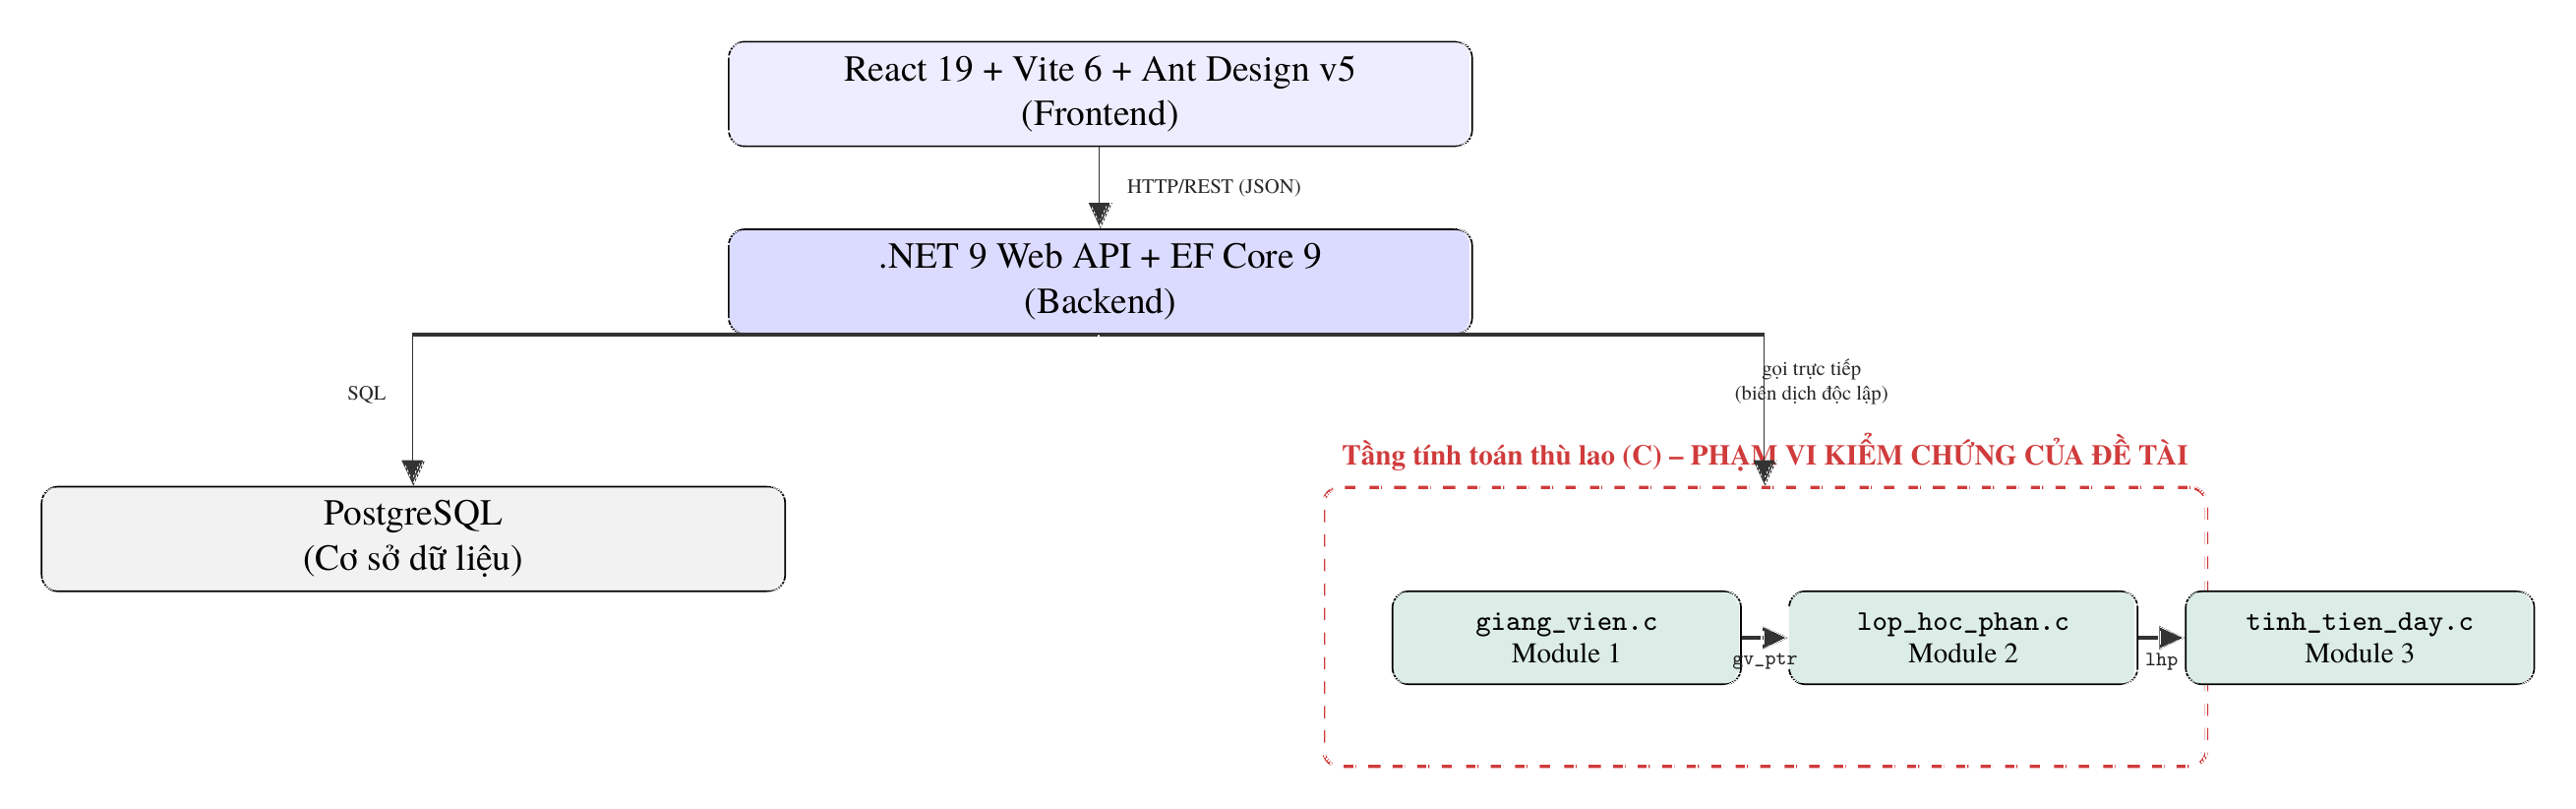
\includegraphics[width=\linewidth]{diagram6_e2e_architecture.png}
  \caption{Kiến trúc tổng quan DuongUniversity Management System -- tầng tính toán C (viền đỏ nét đứt) biên dịch độc lập với .NET, không được GC/bounds-checking của .NET bảo vệ}
  \label{fig:e2e-arch}
\end{figure}

\Cref{fig:e2e-arch} khớp đúng mô tả bằng chữ ở trên: request từ frontend đi qua backend .NET, backend rẽ 2 nhánh -- một sang PostgreSQL để đọc/ghi dữ liệu bền vững, một gọi trực tiếp vào tầng tính toán C (biên dịch thành thư viện/tiến trình riêng, không chạy trong runtime .NET) để tính thù lao; chính đường rẽ thứ hai này là ranh giới an toàn bị mất tác dụng của .NET, và là lý do 3 module C (viền đỏ) là đối tượng kiểm chứng duy nhất của đề tài.

\subsection{Mô tả 3 module mục tiêu}

\begin{itemize}
  \item \textbf{Module 1 -- Quản lý Giảng viên} (\texttt{giang\_vien.c}/\texttt{.h}): định nghĩa struct \texttt{GiangVien} (\texttt{id}, \texttt{maGiangVien}, \texttt{hoTen}, \texttt{bangCap}, \texttt{heSoBangCap}, \texttt{is\_deleted}) và cặp hàm \texttt{add\_lecturer\_VULN()}/\texttt{add\_lecturer\_SAFE()}, \texttt{delete\_lecturer\_VULN()}/\texttt{delete\_lecturer\_SAFE()}.
  \item \textbf{Module 2 -- Quản lý Lớp học phần} (\texttt{lop\_hoc\_phan.c}/\texttt{.h}): định nghĩa struct \texttt{LopHocPhan} (\texttt{id}, \texttt{maLop}, \texttt{soTiet}, \texttt{heSoHocPhan}, \texttt{soLuongSinhVien}, và đặc biệt \textbf{\texttt{gv\_ptr}} -- con trỏ thô trỏ sang \texttt{GiangVien}, chính là điểm liên kết xuyên module tạo ra rủi ro CWE-416/476) và cặp hàm \texttt{create\_class\_section\_VULN()}/\texttt{\_SAFE()}.
  \item \textbf{Module 3 -- Tính tiền dạy \& Thanh toán} (\texttt{tinh\_tien\_day.c}/\texttt{.h}): định nghĩa struct \texttt{Config} (\texttt{heSoQuyMoLop}, \texttt{dinhMucTienChuan}, \texttt{nam}) và 3 cặp hàm \texttt{calculate\_e2e\_salary\_VULN()}/\texttt{\_SAFE()}, \texttt{export\_report\_VULN()}/\texttt{\_SAFE()}, \texttt{pack\_class\_size\_byte\_VULN()}/\texttt{\_SAFE()} -- hàm cuối đóng gói \texttt{soLuongSinhVien} vào bản ghi audit log dạng \texttt{char}.
\end{itemize}

\noindent\textit{Lưu ý:} field \texttt{Config.heSoQuyMoLop} được \textbf{khai báo nhưng không hề được đọc} bởi \texttt{tinh\_tien\_day.c} -- hệ số quy mô lớp thật sự dùng trong công thức dưới đây được tính lại từ \texttt{soLuongSinhVien} (xem statement tường minh tại \Cref{sec:params}), không lấy từ field này. Đây là một field ``chết'' (dead field) phát hiện được khi đối chiếu lại công thức thật với mô hình Z3 ở Chương 3.

\Cref{lst:gvstruct,lst:lhpstruct} trích \emph{nguyên văn} định nghĩa 2 struct cốt lõi từ chính mã nguồn thật của đề tài -- trường \texttt{gv\_ptr} (con trỏ thô, không đếm tham chiếu) chính là điểm liên kết xuyên module tạo ra CWE-416/476 đã nêu.

\lstinputlisting[language=C,firstline=7,lastline=14,caption={Struct \texttt{GiangVien} -- trích nguyên văn \texttt{giang\_vien.h} (dòng 7--14)},label={lst:gvstruct}]{code/giang_vien.h}

\lstinputlisting[language=C,firstline=9,lastline=17,caption={Struct \texttt{LopHocPhan} -- trích nguyên văn \texttt{lop\_hoc\_phan.h} (dòng 9--17)},label={lst:lhpstruct}]{code/lop_hoc_phan.h}

Công thức tính tiền dạy gồm 2 bước, giữ nguyên 100\% giữa bản VULN và bản SAFE (chỉ khác kiểu dữ liệu):
\begin{align*}
  \text{heSoQuyMo} &= (\text{soLuongSinhVien} > 50)\ ?\ 0.2 : 0.0 \\
  \text{soTietQuyDoi} &= \text{soTiet} \times (\text{heSoHocPhan} + \text{heSoQuyMo}) \\
  \text{tienDay} &= \text{soTietQuyDoi} \times \text{gv\_ptr}.\text{heSoBangCap} \times \text{dinhMucTienChuan}
\end{align*}

\subsection{Sơ đồ quan hệ struct (ERD)}

\Cref{fig:erd} thể hiện quan hệ giữa 3 struct và các trường dữ liệu liên quan trực tiếp tới một CWE cụ thể (tô đỏ), đối lập với trường \texttt{dinhMucTienChuan} dùng kiểu \texttt{long long} (int64) đã được chứng minh an toàn (tô xanh, xem Check 2, \Cref{sec:ch3}).

\begin{figure}[H]
  \centering
  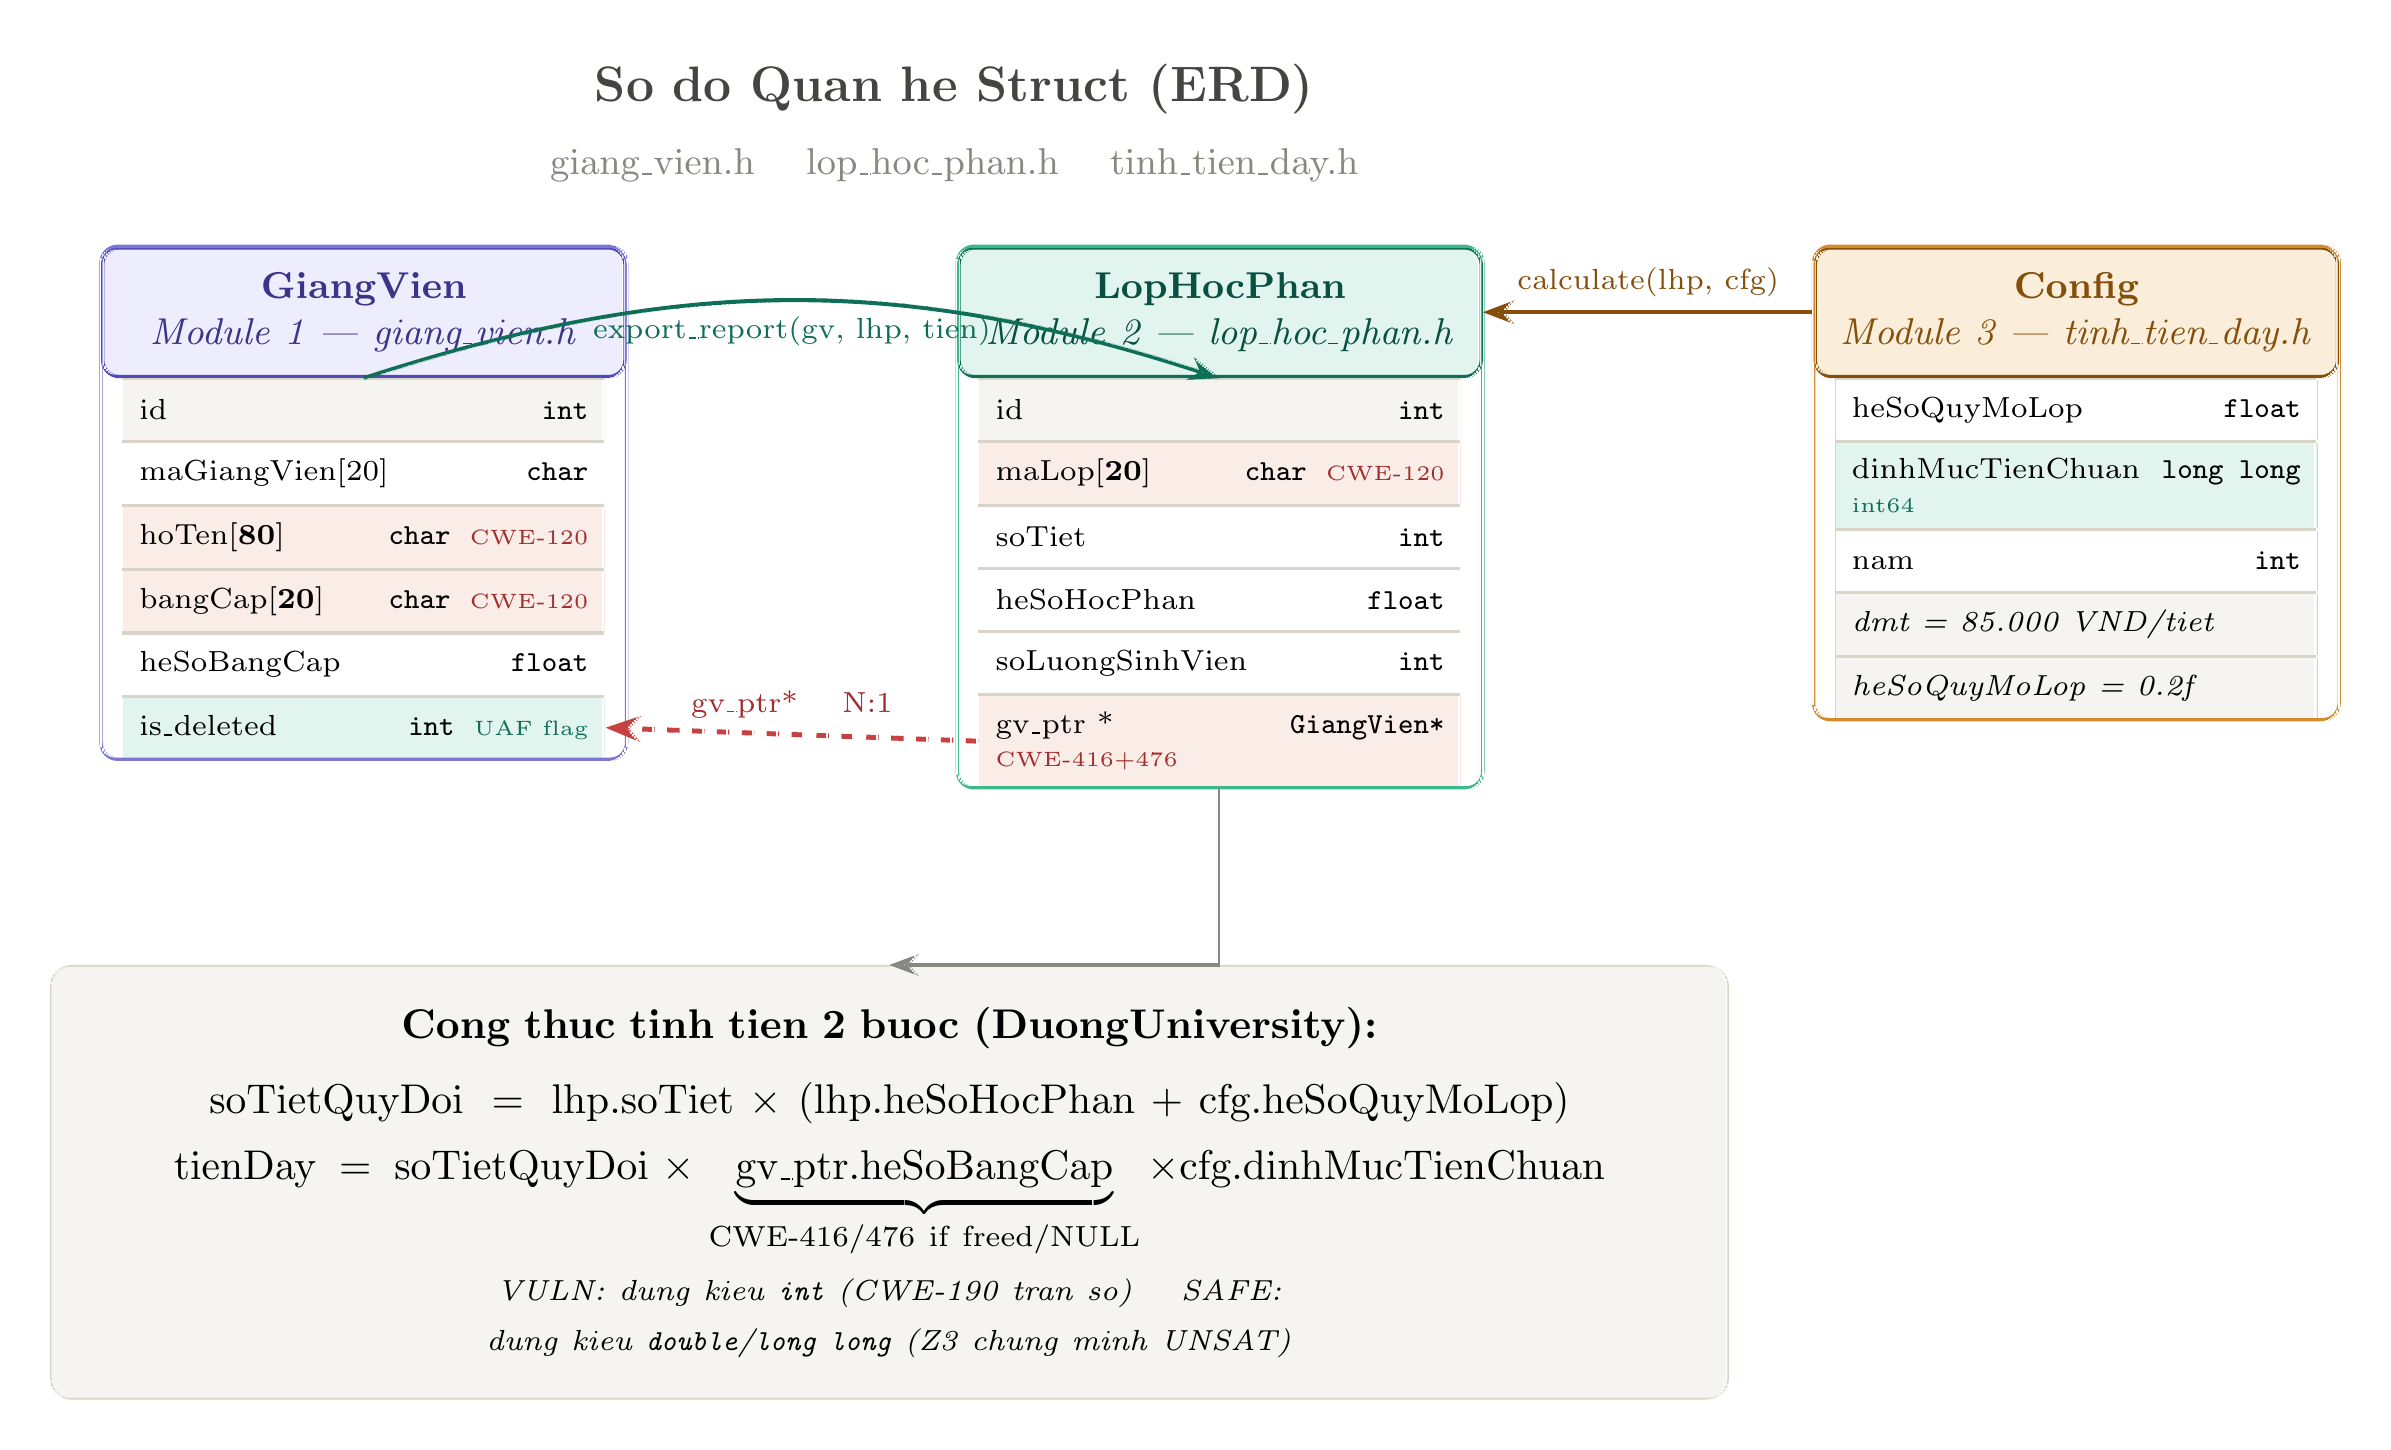
\includegraphics[width=0.95\linewidth]{diagram2_entity_relationship.png}
  \caption{Sơ đồ quan hệ 3 struct \texttt{GiangVien}, \texttt{LopHocPhan}, \texttt{Config} và các trường liên quan tới CWE-120/416/476/190}
  \label{fig:erd}
\end{figure}

\subsection{Sơ đồ luồng dữ liệu (DFD)}

\Cref{fig:dfd} theo dõi dữ liệu từ \texttt{stdin} (không tin cậy) qua Module 1, Module 2, tới Module 3, đánh dấu đúng vị trí mã nguồn (tên file, số dòng) nơi mỗi lỗ hổng CWE-120/416/190/476 phát sinh, cùng kết quả đối chứng của Chương 3 (Z3) và Chương 4 (fuzzing) ngay trên sơ đồ.

\begin{figure}[H]
  \centering
  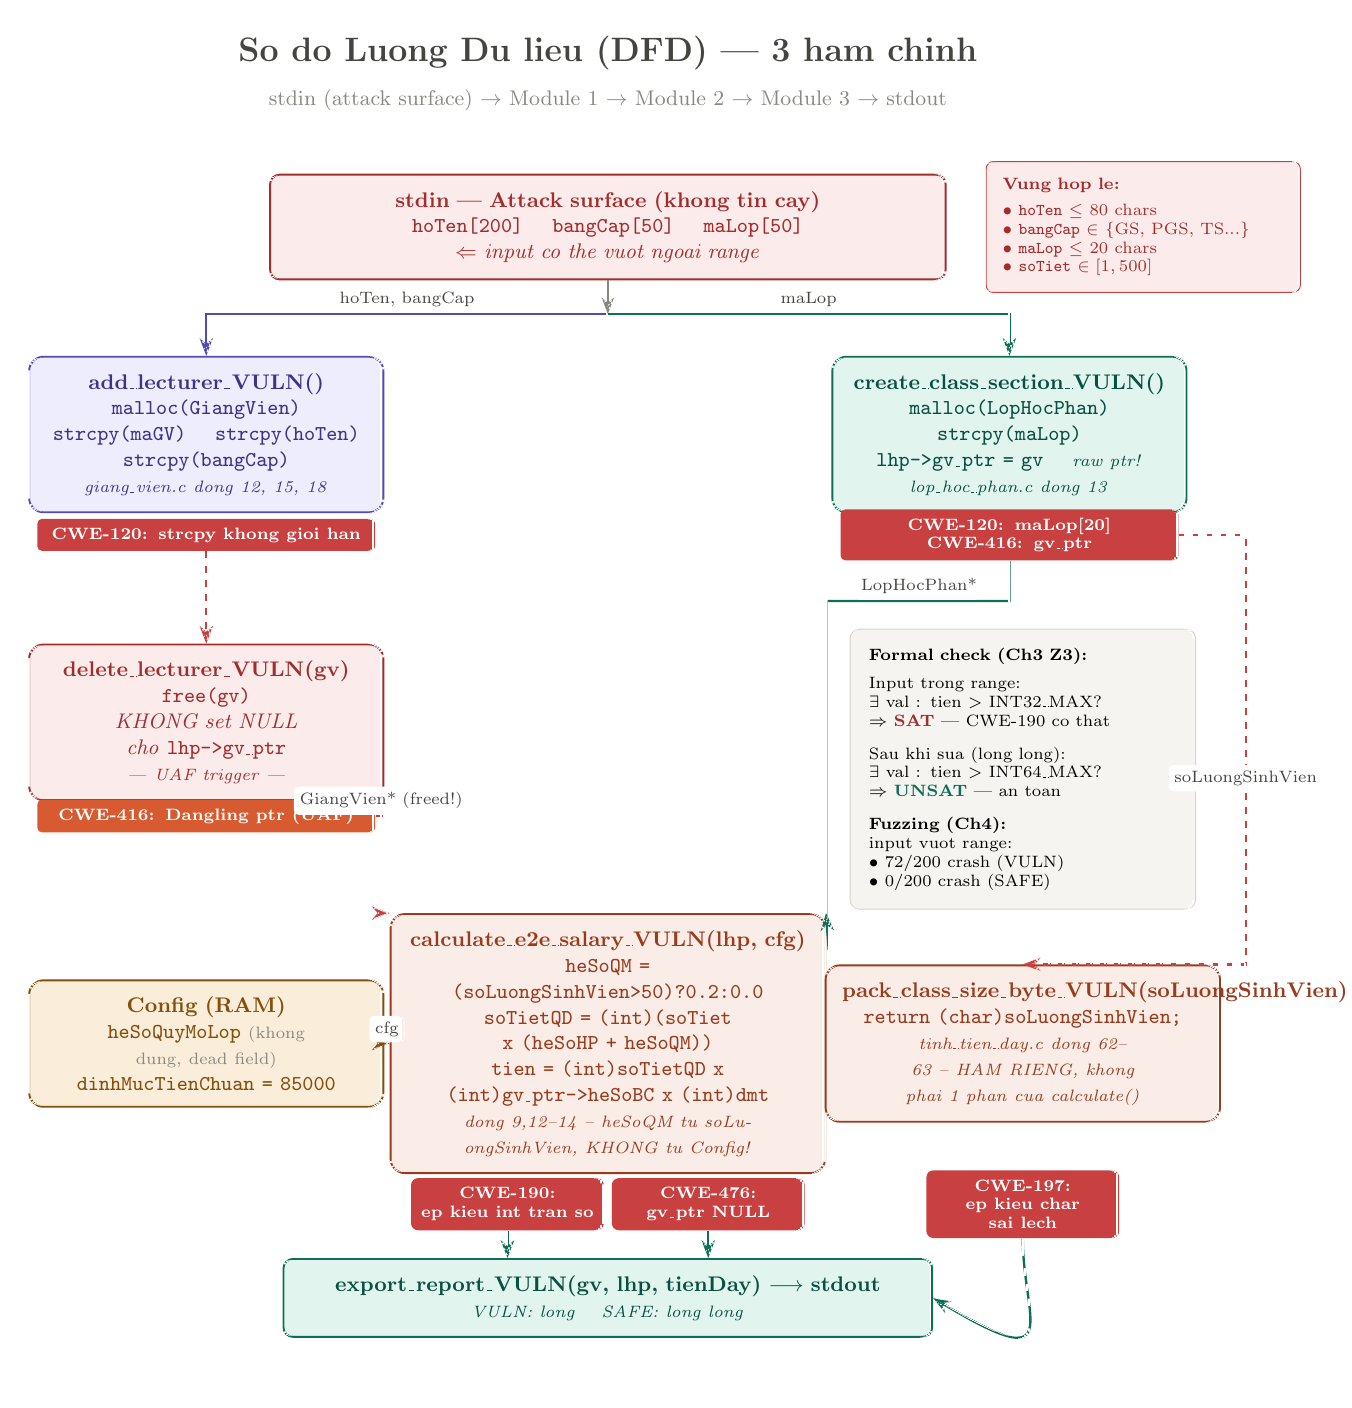
\includegraphics[width=\linewidth]{diagram3_data_flow.png}
  \caption{Sơ đồ luồng dữ liệu qua 3 hàm chính, đánh dấu vị trí phát sinh CWE và kết quả đối chứng Z3/fuzzing}
  \label{fig:dfd}
\end{figure}

\noindent\textit{Lưu ý:} Hai sơ đồ trên được dựng ở giai đoạn đầu của đề tài, khi hệ thống mới có 4 lỗ hổng CWE-120/416/190/476. Lỗ hổng thứ 5 (CWE-1288) và thứ 6 (CWE-197, cùng biến thể ``trùng lặp byte'' của nó) được bổ sung sau nên chưa xuất hiện trên hai hình trên -- được trình bày đầy đủ bằng sơ đồ trạng thái tại \Cref{sec:ch1} (nhãn \texttt{byte\_truncated}) và bảng kết quả tại \Cref{sec:ketqua}.

\subsection{Attack surface}

\begin{itemize}
  \item \texttt{stdin}: \texttt{hoTen} (buffer nhận 200 byte) được \texttt{strcpy} vào \texttt{hoTen[80]} không kiểm tra độ dài -- \textbf{CWE-120}.
  \item \texttt{bangCap} nhập từ \texttt{stdin} không được validate nghiêm ngặt ở bản VULN, rơi vào hệ số mặc định $1.0$ khi sai -- \textbf{CWE-1288}.
  \item \texttt{gv\_ptr} là con trỏ thô xuyên module, không có cơ chế đếm tham chiếu hay huỷ liên kết tự động khi \texttt{GiangVien} bị \texttt{free()} -- \textbf{CWE-416/CWE-476}.
  \item Phép nhân \texttt{soTietQuyDoi} $\times$ \texttt{heSoBangCap} $\times$ \texttt{dinhMucTienChuan} thực hiện trên kiểu \texttt{int} 32-bit ở bản VULN -- \textbf{CWE-190}.
  \item \texttt{soLuongSinhVien} (int, có thể tới vài trăm với lớp đại cương) bị ép kiểu xuống \texttt{char} không kiểm tra phạm vi khi đóng gói audit log -- \textbf{CWE-197}.
\end{itemize}

\subsection{Kích thước/độ phức tạp}

Hệ thống mục tiêu gồm \textbf{520 dòng mã C} (bao gồm cả header) chia trong \textbf{3 file module + 2 file driver} (\texttt{main.c} cho bản VULN, \texttt{main\_fixed.c} cho bản SAFE, dùng chung 3 module), với \textbf{12 hàm chính} (6 hàm \texttt{\_VULN} đối xứng 1-1 với 6 hàm \texttt{\_SAFE}), tạo điều kiện để mọi bản vá đều có thể so sánh trực tiếp hành vi trước/sau trên cùng một lời gọi hàm.
